\documentclass{standalone}
\usepackage{mathpazo}
\usepackage{siunitx}
\usepackage[american voltages, american currents, american inductors]{circuitikz}
\newcommand*{\equal}{=}

\begin{document}
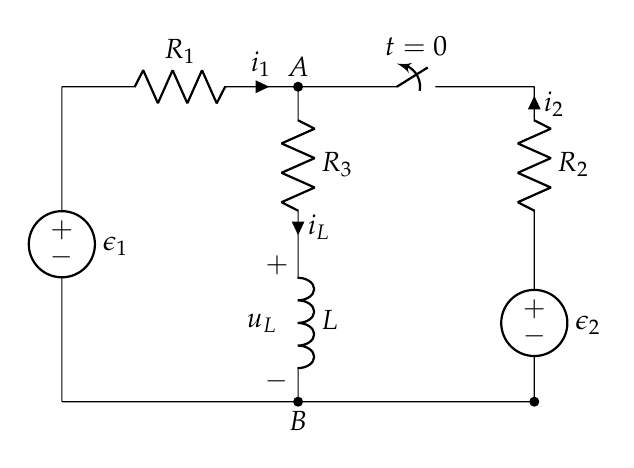
\begin{tikzpicture}
  \coordinate (A) at (0,4);
  \coordinate (B) at (3,4);
  \coordinate (C) at (6,4);
  \coordinate (D) at (0,0);
  \coordinate (E) at (3,0);
  \coordinate (F) at (6,0);
  \draw
  (A) to [R, l = $R_1$, i = $i_1$, -*] (B) node[above] {$A$}
  to [opening switch, l = $t \equal 0$] (C)
  (D) to [short, -*] (E) node[below] {$B$}
  to [short, -*] (F)
  (A) to [V, l = $\epsilon_1$] (D)
  (B) to [R, l = $R_3$, i = $i_L$] ++(0, -2)
  to [L, l = $L$, v = $u_L$] (E)
  (C) to [R, l = $R_2$, i<= $i_2$] ++(0,-2)
  to [V, l = $\epsilon_2$] (F);
  \end{tikzpicture}
\end{document}